\documentclass[12pt]{article}
\usepackage{graphics,textcomp}
\newcommand{\micro}{\hbox{\textmu}}
\newcommand{\unit}[1]{\mathrm{#1}}
  \renewcommand{\deg}{\unit{deg}}
  \newcommand{\rad}{\unit{rad}}
  \newcommand{\s}{\unit{s}}
  \newcommand{\ns}{\unit{ns}}
  \newcommand{\m}{\unit{m}}
    \newcommand{\mps}{\m\,\s^{-1}}
  \newcommand{\cm}{\unit{cm}}
  \newcommand{\mm}{\unit{mm}}
  \newcommand{\mum}{\unit{\micro m}}
  \newcommand{\nm}{\unit{nm}}
  \newcommand{\kg}{\unit{kg}}
  \newcommand{\g}{\unit{g}}
  \newcommand{\Hz}{\unit{Hz}}
  \newcommand{\N}{\unit{N}}
  \newcommand{\V}{\unit{V}}
    \newcommand{\Vpm}{\V\,\m^{-1}}
  \newcommand{\C}{\unit{C}}
\newcommand{\dd}{\mathrm{d}}
\newcounter{answer}
\newenvironment{alist}{\begin{list}{(\Alph{answer})}{\usecounter{answer}}}%
  {\end{list}}
% \newcommand{\explicitcorrect}[1]{[({#1})~\textbf{correct}]}
\newcommand{\correct}{~[\textbf{correct}]}
\newcommand{\source}[1]{\textsl{#1}}
\renewcommand{\emph}[1]{\textbf{#1}}
\begin{document}
\raggedright
\begin{enumerate}

\item (from lecture 2009-02-11) A microscope is made up of two
  converging lenses, the objective and the eyepiece.  If a scientist
  is looking at a sample in focus in the microscope, which of the
  following is \emph{true}?
  \begin{alist}
  \item There is a real, inverted image between the objective and the
    eyepiece.\correct
  \item There is a real, non-inverted image between the objective and
    the eyepiece.
  \item There are only virtual images inside the microscope.
  \item There no images at all inside the microscope.
  \end{alist}

\item (from lecture 2009-02-11) In a microscope, the optics have the
  following property:
  \begin{alist}
  \item if the objective has a shorter focal length, the magnification
    will be higher.\correct
  \item if the objective has a longer focal length, the magnification
    will be higher.
  \item the objective and the eyepiece ought to have very similar
    focal lengths.
  \item the focal length of the objective should be much longer than
    the focal length of the eyepiece.
  \item none of the above
  \end{alist}

\item (from Chapter 26) Which of the following systems has the largest
  magnitude of positive charge?
  \begin{alist}
  \item 1 proton
  \item 1 electron
  \item 17 protons + 21 electrons
  \item 1,000,000 protons + 1,000,000 electrons
  \item a $12\,\g$ ball of carbon missing 3 electrons\correct
  \end{alist}

\item (from lecture 2009-02-18) If you gave one mole of
  your electrons to your friend, who is standing $1\,\m$ away from
  you, what attractive electrical force would you feel?
  \begin{alist}
  \item $10^{14}\,\N$
  \item $10^{17}\,\N$
  \item $10^{20}\,\N$\correct
  \item far less than any of those
  \item far greater than any of those
  \end{alist}

\item (from lecture 2009-02-18) How do we know that the Universe is
  very close to being electrically neutral?
  \begin{alist}
  \item we would see more lightning if it wasn't
  \item the stars would be brighter if it wasn't
  \item electrical forces would be stronger than gravitational forces
    if it wasn't\correct
  \item water molecules would align with the local electrical field if
    it wasn't
  \item we \emph{don't} know that the Universe is close to neutral
  \end{alist}

\item (from conceptual question 26.14) An ion of charge $+4\,e$ and an
  electron of charge $-e$ are in an evacuated part of outer space,
  instantaneously separated by a distance of $1\,\cm$.  Where is there
  a position at which a \emph{nearby} test charge would experience no
  electrical force at this moment in time?
  \begin{alist}
  \item There is no such location.
  \item There is a location and it is in between the two charges.
  \item There is a location \emph{not} between the two charges, closer
    to the electron than the ion.\correct
  \item There is a location \emph{not} between the two charges, closer
    to the ion than the electron.
  \end{alist}

\item (from lecture 2009-02-23) Imagine a glass that holds $1.000$\,pint of
  beer.  Now increase all its linear dimensions (its radius and
  height) by one percent, making a very similar-shaped glass but just
  very slightly larger.  How much beer does the new glass hold?
  \begin{alist}
  \item 1.001\,pint
  \item 1.003\,pint
  \item 1.010\,pint
  \item 1.030\,pint\correct
  \item none of the above
  \end{alist}

\item (from lecture 2009-02-23) The electric field of a dipole falls
  as the cube of the distance or $1/r^3$.  This is only approximately
  true, and only when
  \begin{alist}
  \item the distance is much greater than the separation of the
    charges in the dipole\correct
  \item the charges are very small
  \item the dipole is aligned with an external electric field
  \end{alist}

\item (from Chapter 26+27 homework) What is the magnitude $E$ of an
  upward-directed electric field that will exactly cancel the
  gravitational force $m\,g$ from the Earth on a proton?
  \begin{alist}
  \item $\displaystyle\frac{e}{4\pi\,\epsilon_0\,m\,g}$
  \item $\displaystyle\frac{e}{4\pi\,\epsilon_0\,r_E^2}$, where $r_E$ is Earth's radius
  \item $\displaystyle\frac{m\,g}{e}$\correct
  \item $\displaystyle\frac{q\,E}{m\,g}$
  \item none of the above
  \end{alist}

\item (from lecture 2009-03-02) Which of the following integrals would
  integrate to the magnitude of the electric field a perpendicular
  distance $b$ from an infinitely long, straight wire with charge per
  unit length $\lambda$?
  \begin{alist}
  \item $\displaystyle\frac{1}{4\pi\,\epsilon_0}
         \,\int_{-\infty}^{\infty} \frac{\lambda\,\dd x}{[x^2 + b^2]^{3/2}}$
  \item $\displaystyle\frac{1}{4\pi\,\epsilon_0}
         \,\int_{-\infty}^{\infty} \frac{\lambda\,\dd x}{[x^2 + b^2]}$
  \item $\displaystyle\frac{1}{4\pi\,\epsilon_0}
         \,\int_{-\infty}^{\infty} \frac{\lambda\,b\,\dd x}{[x^2 + b^2]}$
  \item $\displaystyle\frac{1}{4\pi\,\epsilon_0}
         \,\int_{-\infty}^{\infty} \frac{\lambda\,b\,\dd x}{[x^2 + b^2]^{3/2}}$\correct
  \item none of the above
  \end{alist}

\item (from lecture 2009-03-02) Inside a charged capacitor, which
  statement is closest to being true?
  \begin{alist}
  \item the electric field is parallel to the plates, and the
    equipotentials are perpendicular to the plates
  \item both the electric field and the equipotentials are parallel to
    the plates
  \item both the electric field and the equipotentials are
    perpendicular to the plates
  \item the electric field is perpendicular to the plates and the
    equipotentials are parallel to the plates\correct
  \end{alist}

\item (from conceptual question 27.15) A proton and electron are
  released from rest inside a charged, parallel-plate capacitor.
  Which statement is true?
  \begin{alist}
  \item They experience equal-magnitude forces, but the proton has a
    larger magnitude acceleration.
  \item They experience equal-magnitude forces, but the proton has a
    smaller magnitude acceleration.\correct
  \item They experience equal-magnitude accelerations, but the proton
    experiences a larger magnitude force.
  \item They experience equal-magnitude accelerations, but the proton
    experiences a smaller magnitude force.
  \item They experience equal-magnitude accelerations, and
    equal-magnitude forces.
  \end{alist}

\item (from exercise 27.19) Air breaks down when the electric field
  strength gets to be $3\times 10^6\,\Vpm$.  A parallel-plate
  capacitor with two plates of area $0.020\,\m^2$ is charged up by
  moving charge $Q$ from one plate to the other.  At what charge $Q$
  does the air break down and a spark jumps the gap?
  \begin{alist}
  \item it depends on the separation between the plates
  \item $6\times 10^{-20}\,\C$
  \item $5\times 10^{-7}\,\C$\correct
  \item $7\times 10^{-6}\,\C$
  \item $2\times 10^{6}\,\C$
  \end{alist}

\item (from Chapter 27 homework) A charge $q$ of mass $m$ is moving at
  speed $v_y$ in the $y$ direction.  It passes through a uniform
  electric field $E$ acting in the $x$ direction.  This electric field
  exists only in a region of space of $y$-direction length $L$.  What
  is the $x$-direction velocity component $v_x$ after it has passed
  through this field?
  \begin{alist}
  \item $0$
  \item $\displaystyle\frac{q\,E\,L}{m\,v_y}$\correct
  \item $\displaystyle 2\,\frac{m}{q}\,\left[\frac{v_y}{L}\right]^2$
  \item $\displaystyle\frac{L}{v_y}$
  \item none of the above
  \end{alist}

\item (from exercise 27.25) The permanent dipole moment of a water
  molecule is $6.2\times 10^{-30}\,\C\,\m$.  What is the maximum
  possible torque on a water molecule in an electric field of strength
  $3\times 10^6\,\Vpm$?
  \begin{alist}
  \item $2\times 10^{-36}\,\N\,\m$
  \item $2\times 10^{-23}\,\N\,\m$\correct
  \item $5\times 10^{22}\,\N\,\m$
  \item $5\times 10^{35}\,\N\,\m$
  \item nowhere near any of those
  \end{alist}

\item (from lecture 2009-03-02) Which of the following expressions
  could be an expression for the electric potential?  Assume $Q$ is a
  charge, $d$ is a length, and $A$ is an area.
  \begin{alist}
  \item $\displaystyle\frac{1}{4\pi\,\epsilon_0}\,\frac{Q^2}{d}$
  \item $\displaystyle\frac{1}{4\pi\,\epsilon_0}\,\frac{Q}{d^2}$
  \item $\displaystyle\frac{Q}{\epsilon_0\,A}$
  \item $\displaystyle\frac{Q\,d}{\epsilon_0\,A}$\correct
  \item none of the above
  \end{alist}

\item (from lecture 2009-03-04) What happens to a free dipole in a
  non-uniform electric field?
  \begin{alist}
  \item It will rotate to align with the electric field and then be
    attracted to the region of higher field amplitude.\correct
  \item It will rotate to align with the electric field and then be
    repulsed from the region of higher field amplitude.
  \item It will rotate to align with an equipotential surface and then
    be attracted to the region of higher field amplitude.
  \item It will rotate to align with an equipotential surface and then
    be repulsed from the region of higher field amplitude.
  \item None of the above.
  \end{alist}

\item (from lecture 2009-03-04) What happens to a pair of free dipoles
  in a region with no other sources of electric field?
  \begin{alist}
  \item They tend to rotate to point in the same direction and feel an attractive force.\correct
  \item They tend to rotate to point in opposite directions and feel an attractive force.\correct
  \item They tend to rotate to point in the same direction and feel a repulsive force.
  \item They tend to rotate to point in opposite directions and feel a repulsive force.
  \item They do not interact because they are neutral.
  \end{alist}

\item (from Chapter 29+30 homework) In the figure below, what can you
  say about the change in electric potential going from the point
  marked ``c'' to the point marked
  ``b''?\\ \resizebox{2in}{!}{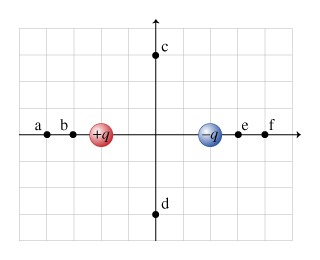
\includegraphics{1011435.jpg}}\\
  \begin{alist}
  \item the potential increases from c to b\correct
  \item the potential decreases from c to b
  \item the potential is the same at c and b
  \item the change in potential depends on the sign of the test charge used
  \item the change in potential depends on the path you take
  \end{alist}

\item (from exercise 29.18) The two contacts of an AA battery
  ($1.5\,\V$) are connected to the two plates of a parallel-plate
  capacitor with a plate area of $0.020\,\m^2$ and plate separation of
  $0.001\,\m$.  How much charge does the battery maintain on each
  plate?
  \begin{alist}
  \item $2.6\times 10^{-16}\,\C$
  \item $6.6\times 10^{-13}\,\C$
  \item $2.6\times 10^{-10}\,\C$\correct
  \item $6.6\times 10^{-7}\,\C$
  \item nowhere near any of these
  \end{alist}

\end{enumerate}
\end{document}
